% % % % % % % % % % % % % % % % % % % % % % % % % % % % % % % % % % % % % % % % % % % %
%                                                                                     %
% Short Sectioned Assignment LaTeX Template Version 1.0 (5/5/12)                      %
% This template has been downloaded from: http://www.LaTeXTemplates.com               %
%                                                                                     %
% Original author:  Frits Wenneker (http://www.howtotex.com)                          %
%                                                                                     %
% Modified by: Fco Javier Sueza Rodríguez (fcosueza@disroot.org)                      %
%                                                                                     %
% Changes:                                                                            %
%	    - Custom Chapters, Sections and Subsections (titlesec package)                %
%           - Document type scrbook (oneside)                                         %
%           - Use babel-lang-spanish package and marvosym                             %
%           - Use hyperref, enumitem, tcolorbox and glossaries packages               %
%           - Use Time New Roman (mathptmx), Helvetic and Courier fonts               %
%                                                                                     %
% License: CC BY-NC-SA 3.0 (http://creativecommons.org/licenses/by-nc-sa/3.0/)        %
%                                                                                     %
% % % % % % % % % % % % % % % % % % % % % % % % % % % % % % % % % % % % % % % % % % % %

%-----------------------------------------------%
%	              Packages                  %
%-----------------------------------------------%

\documentclass[paper=a4, fontsize=11pt, oneside]{scrbook}

% ---- Text Input/Output ----- %

\usepackage[T1]{fontenc}
\usepackage[utf8]{inputenc}
\usepackage{mathptmx}
\usepackage[scaled=.92]{helvet}
\usepackage{courier}
\usepackage[indent=12pt]{parskip}

\usepackage{geometry}
\geometry{verbose,tmargin=3cm,bmargin=3cm,lmargin=2.6cm,rmargin=2.6cm}

% ---- Language ----- %

\usepackage[spanish]{babel}
\usepackage{marvosym}

% ---- Another packages ---- %

\usepackage{amsmath,amsfonts,amsthm}
\usepackage{graphics,graphicx}
\usepackage{titlesec}
\usepackage{fancyhdr}
\usepackage{tcolorbox}
\usepackage{hyperref}
\usepackage{enumitem}
\usepackage[automake]{glossaries}

%--------------------------------------------------------------------%
%                      Customizing Document                          %
%--------------------------------------------------------------------%


% ----------- Custom Chapters, Sections and Subsections -------------- %

\titleformat{\chapter}[display]
			{\bfseries\Huge}
			{Tema \ \thechapter} {0.5ex}
			{\vspace{1ex}\centering}

\titleformat{\section}[hang]
			{\bfseries\Large}
			{\thesection}{0.5em}{}

\titleformat{\subsection}[hang]
			{\bfseries\large}
			{\thesubsection}{0.5em}{}

\titleformat{\subsubsection}[hang]
			{\bfseries\large}
			{\thesubsubsection}{0.5em}{}

\hypersetup{
    colorlinks=true,
    linkcolor=black,
    urlcolor=magenta
}

% ------------------- Custom heaaders and footers ------------------- %

\pagestyle{fancyplain}

\fancyhead[]{}
\fancyfoot[L]{}
\fancyfoot[C]{}
\fancyfoot[R]{\thepage}

\renewcommand{\headrulewidth}{0pt} % Remove header underlines
\renewcommand{\footrulewidth}{0pt} % Remove footer underlines

\setlength{\headheight}{13.6pt} % Customize the height of the header

% --------- Numbering equations, figures and tables ----------------- %

\numberwithin{equation}{section} % Number equations within sections
\numberwithin{figure}{section} % Number figures within sections
\numberwithin{table}{section} % Number tables within sections

% ------------------------ New Commands ----------------------------- %

\newcommand{\horrule}[1]{\rule{\linewidth}{#1}} % Create horizontal rule command


%----------------------------------------------------------------------------------------
%	TÍTULO Y DATOS DEL ALUMNO
%----------------------------------------------------------------------------------------

\title{
\vspace{10ex}
\normalfont \normalsize
\huge \textbf{Actividades de la Unidad 2}
}
\author{Francisco Javier Sueza Rodríguez}
\date{\normalsize\today}

%----------------------------------------------------------------------------------------
%                                     DOCUMENTO
%----------------------------------------------------------------------------------------
\begin{document}

\maketitle

\thispagestyle{empty}

\vspace{75ex}

\begin{center}
    \begin{tabular}{l l}
        \textbf{Centro}: & IES Aguadulce \\
        \textbf{Ciclo Formativo}: & Desarrollo Aplicaciones Web (Distancia)\\
        \textbf{Asignatura}: & Formación y Orientación Laboral\\
        \textbf{Tema}: & Tema 2 -  La Relación Colectiva en el Trabajo\\
    \end{tabular}
\end{center}

\newpage

\section{Actividad 1}
\subsection{Enunciado}
Seguro que has oído hablar del teletrabajo o estás trabajando así. Te invitamos a una reflexión sobre las ventajas y desventajas desde el punto de vista del trabajador.

\subsection{Respuesta}
El \textbf{teletrabajo} es una modalidad de trabajo que, especialmente durante la pandemia, a aumentado considerablemente. Esta es una modalidad que tiene, desde mi punto de vista, bastante ventajas y alguno inconvenientes.

Respecto a las \textbf{ventajas}, el teletrabajo ayuda a la conciliación familiar, ya que el realizar el trabajo desde casa podemos pasar más tiempo con la familia, facilitando en los casos que sea necesario cuidar de algunos miembros de la familiar durante más tiempo. Además, según algunos estudios \cite{bussi}, el teletrabajo incrementa la productividad. Algo que tampoco sorprende, ya que ademas de trabajar en un ambiente familiar más distendido, se evitan desplazamientos, que a veces pueden generar estrés, especialmente en grandes ciudades con mucho tráfico en horas concretas.

Por otro lado, el teletrabajo tiene sus \textbf{desventajas}. Por un lado, no todos los puestos de trabajo son susceptibles de ejercer en esta modalidad, hay empleos que son necesariamente presenciales y que no pueden desarrollarse en la distancia, como cualquier empleo en hostelería, dependientes en negocios, trabajos de la construcción, etc. Además, dependiendo de las circunstancias de cada uno en su casa, puede que el ambiente no sea el más adecuado para desarrollar el trabajo, por ejemplo, porque no hay la suficiente tranquilidad para concentrarse. Un factor que tiene también en contra es que se reduce la socialización que si tendríamos acudiendo a la oficina. Aunque hagamos videoconferencias a diario, no es lo mismo que el trato cara a cara con los compañeros.

En definitiva, el teletrabajo tiene sus virtudes y sus defectos, y ya dependerá de cada persona y cada situación si es más o menos idóneo para el correcto desarrollo de las funciones propias del puesto de trabajo.

\section{Actividad 2}
\subsection{Enunciado}

\subsubsection*{La Negociación Colectiva}
Busca un convenio colectivo vigente aplicable al sector profesional de informática, que no esté además tratado o ejemplificado en el tema, y responde justificadamente a las siguientes cuestiones:

\begin{enumerate}
    \item Haz una captura legible en el que se identifique el convenio elegible y añade enlace activo al mismo para que pueda consultarlo.
    \item En cuanto al contenido mínimo del convenio mediante captura muestra el artículo que haga referencia a los siguientes apartado. Es necesario tras la captura copiar la \textbf{información pedida}:
    \begin{enumerate}
        \item Indicación de las partes que lo han negociado.
        \item Ámbito de aplicación personal, funcional, territorial y temporal
    \end{enumerate}
    \item Realiza una captura referente a la planificación anual de las vacaciones y copia debajo el texto.
    \item Busca un artículo del convenio que te llame la atención (por interés ,curiosidad, desacuerdo..etc) sobre algún tipo de contenido:
    \begin{enumerate}
        \item Explica qué tipo de contenido trata
        \item Haz una captura del mismo y copia debajo el artículo capturado.
        \item Justifica tu elección
    \end{enumerate}
\end{enumerate}

\subsection{Respuesta}

\begin{enumerate}
    \item Para esta actividad, se ha elegido el \textbf{XIX Convenio colectivo del sector de empresas de ingeniería y oficinas de estudios técnicos}, uno de los que se puede aplicar a los programadores de aplicaciones informáticas, el cuál se puede encontrar en la \href{https://www.boe.es/diario_boe/txt.php?id=BOE-A-2019-14977}{página del BOE} correspondiente.

    En la siguiente figura de muestra una imagen del encabezado del convenio colectivo.

    \begin{figure}[H]
        \centering
        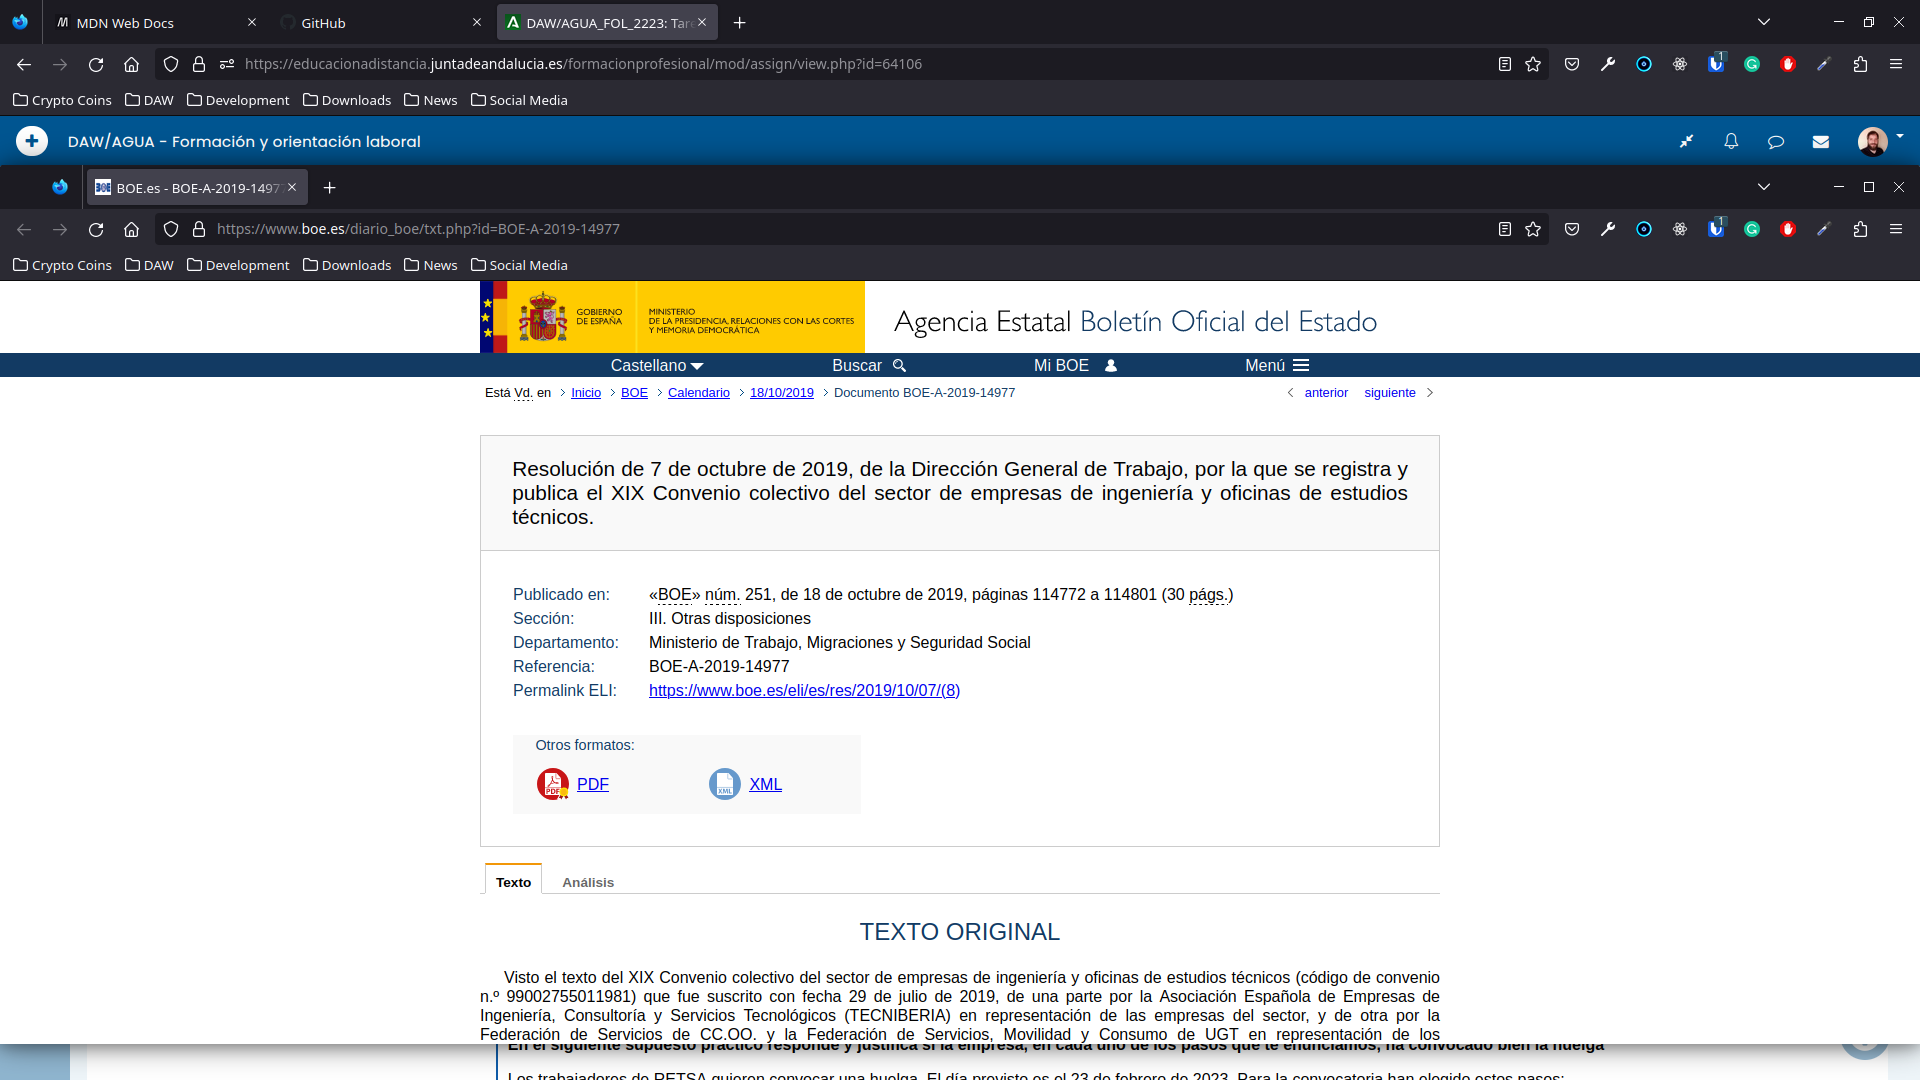
\includegraphics[scale=0.20]{conv-Encabezado.png}
        \caption{Encabezado del convenio colectivo}
    \end{figure}

    \item El contenido mínimo del convenio es el siguiente:
    \begin{enumerate}
        \item El texto, donde se especifican las partes esta en el preámbulo, antes del punto primero, como podemos ver en la siguiente captura:

        \begin{figure}[H]
            \centering
            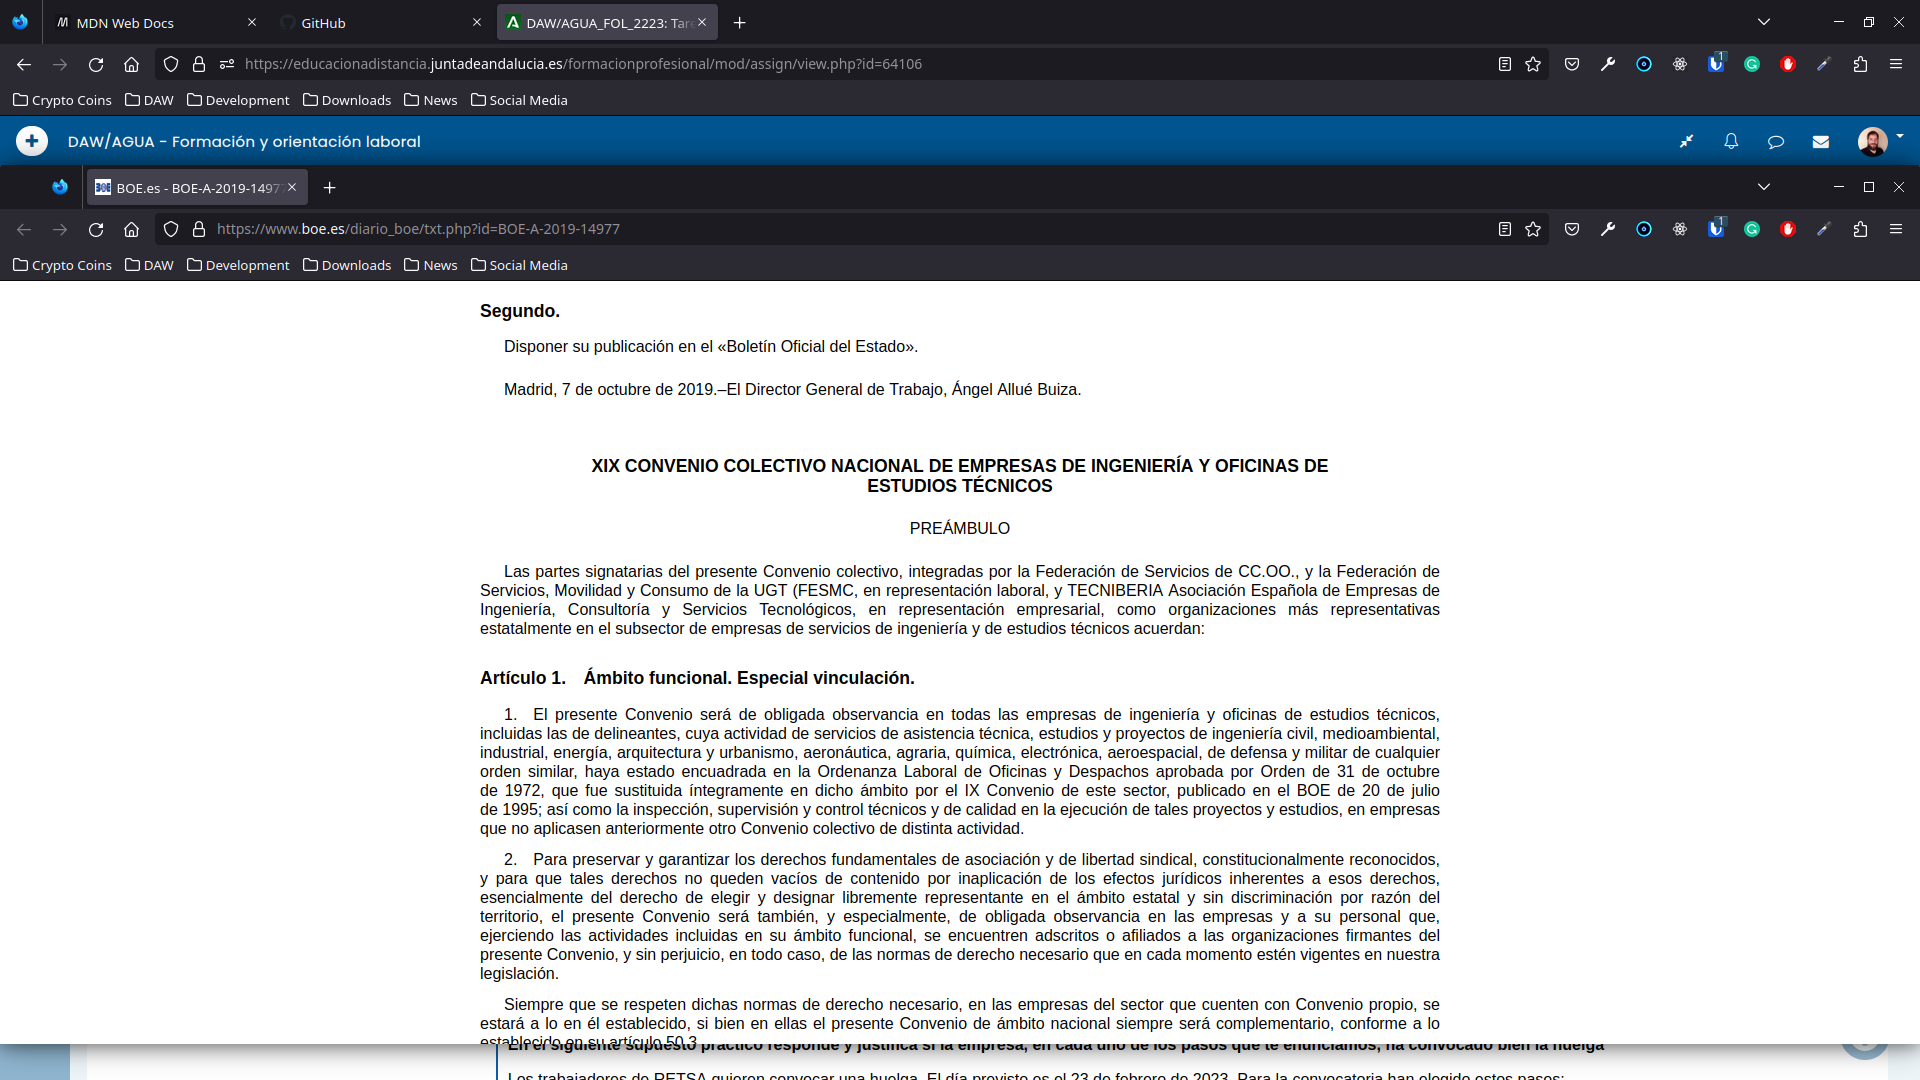
\includegraphics[scale=0.20]{conv-Partes.png}
            \caption{Partes negociadoras en el convenio}
        \end{figure}

        El \textbf{texto} de este punto es el siguiente:

         ``Las partes signatarias del presente Convenio colectivo, integradas por la Federación de Servicios de CC.OO., y la Federación de Servicios, Movilidad y Consumo de la UGT (FESMC, en representación laboral, y TECNIBERIA Asociación Española de Empresas de Ingeniería, Consultoría y Servicios Tecnológicos, en representación empresarial, como organizaciones más representativas estatalmente en el subsector de empresas de servicios de ingeniería y de estudios técnicos acuerdan''

         \item El ámbito de aplicación del convenio, se especifica en los \textbf{artículos 1, 2 3 y 4}, como vemos en la siguiente captura.

          \begin{figure}[H]
             \centering
             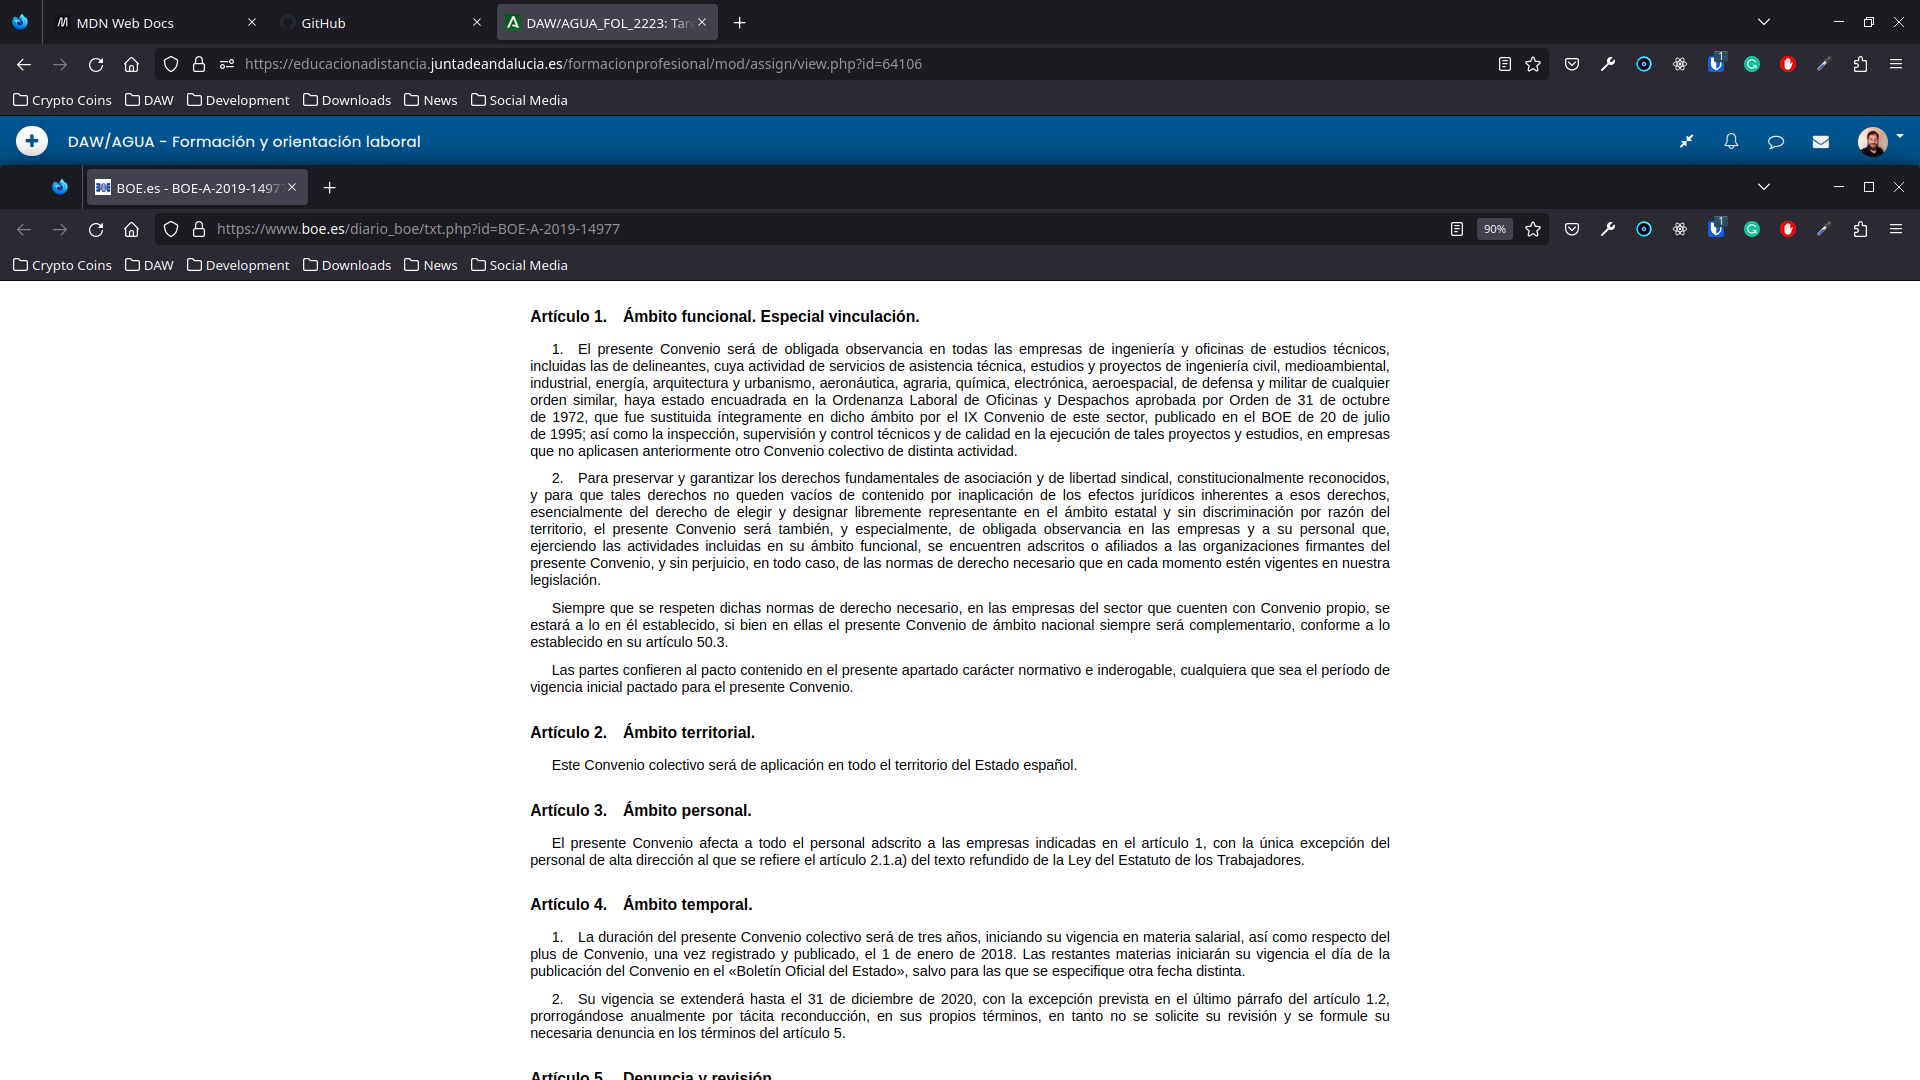
\includegraphics[scale=0.20]{conv-Ambito.png}
             \caption{Ámbito de aplicación del convenio}
         \end{figure}

        Y su \textbf{texto} es el siguiente:

        \begin{itemize}
            \item \textbf{Artículo 1. Ámbito funcional. Especial vinculación.}

            \begin{enumerate}
                \item El presente Convenio será de obligada observancia en todas las empresas de ingeniería y oficinas de estudios técnicos, incluidas las de delineantes, cuya actividad de servicios de asistencia técnica, estudios y proyectos de ingeniería civil, medioambiental, industrial, energía, arquitectura y urbanismo, aeronáutica, agraria, química, electrónica, aeroespacial, de defensa y militar de cualquier orden similar, haya estado encuadrada en la Ordenanza Laboral de Oficinas y Despachos aprobada por Orden de 31 de octubre de 1972, que fue sustituida íntegramente en dicho ámbito por el IX Convenio de este sector, publicado en el BOE de 20 de julio de 1995; así como la inspección, supervisión y control técnicos y de calidad en la ejecución de tales proyectos y estudios, en empresas que no aplicasen anteriormente otro Convenio colectivo de distinta actividad.

                \item Para preservar y garantizar los derechos fundamentales de asociación y de libertad sindical, constitucionalmente reconocidos, y para que tales derechos no queden vacíos de contenido por inaplicación de los efectos jurídicos inherentes a esos derechos, esencialmente del derecho de elegir y designar libremente representante en el ámbito estatal y sin discriminación por razón del territorio, el presente Convenio será también, y especialmente, de obligada observancia en las empresas y a su personal que, ejerciendo las actividades incluidas en su ámbito funcional, se encuentren adscritos o afiliados a las organizaciones firmantes del presente Convenio, y sin perjuicio, en todo caso, de las normas de derecho necesario que en cada momento estén vigentes en nuestra legislación.
            \end{enumerate}

            Siempre que se respeten dichas normas de derecho necesario, en las empresas del sector que cuenten con Convenio propio, se estará a lo en él establecido, si bien en ellas el presente Convenio de ámbito nacional siempre será complementario, conforme a lo establecido en su artículo 50.3.

            Las partes confieren al pacto contenido en el presente apartado carácter normativo e inderogable, cualquiera que sea el período de vigencia inicial pactado para el presente Convenio.

            \item \textbf{Artículo 2. Ámbito territorial.}

            Este Convenio colectivo será de aplicación en todo el territorio del Estado español.

            \item \textbf{Artículo 3. Ámbito personal.}

             El presente Convenio afecta a todo el personal adscrito a las empresas indicadas en el artículo 1, con la única excepción del personal de alta dirección al que se refiere el artículo 2.1.a) del texto refundido de la Ley del Estatuto de los Trabajadores.

             \item \textbf{Artículo 4. Ámbito temporal.}
             \begin{enumerate}
                 \item La duración del presente Convenio colectivo será de tres años, iniciando su vigencia en materia salarial, así como respecto del plus de Convenio, una vez registrado y publicado, el 1 de enero de 2018. Las restantes materias iniciarán su vigencia el día de la publicación del Convenio en el «Boletín Oficial del Estado», salvo para las que se especifique otra fecha distinta.

                 \item En el caso de solicitarse la revisión del Convenio, la parte que formule su denuncia deberá simultáneamente presentar comunicación de la promoción de la negociación con propuesta concreta sobre los puntos, el contenido mínimo que comprenda la revisión solicitada y requisitos establecidos en el artículo 89.1 del Estatuto de los Trabajadores. Caso de incumplimiento, se tendrá por no hecha la denuncia. De esta comunicación y de la propuesta se enviará copia, a efectos de registro, a la Dirección General de Empleo.
             \end{enumerate}
        \end{itemize}

        \item El texto referente a las vacaciones se encuentra en el \textbf{Articulo 23}, como se muestra en la captura de pantalla.

        \begin{figure}[H]
            \centering
            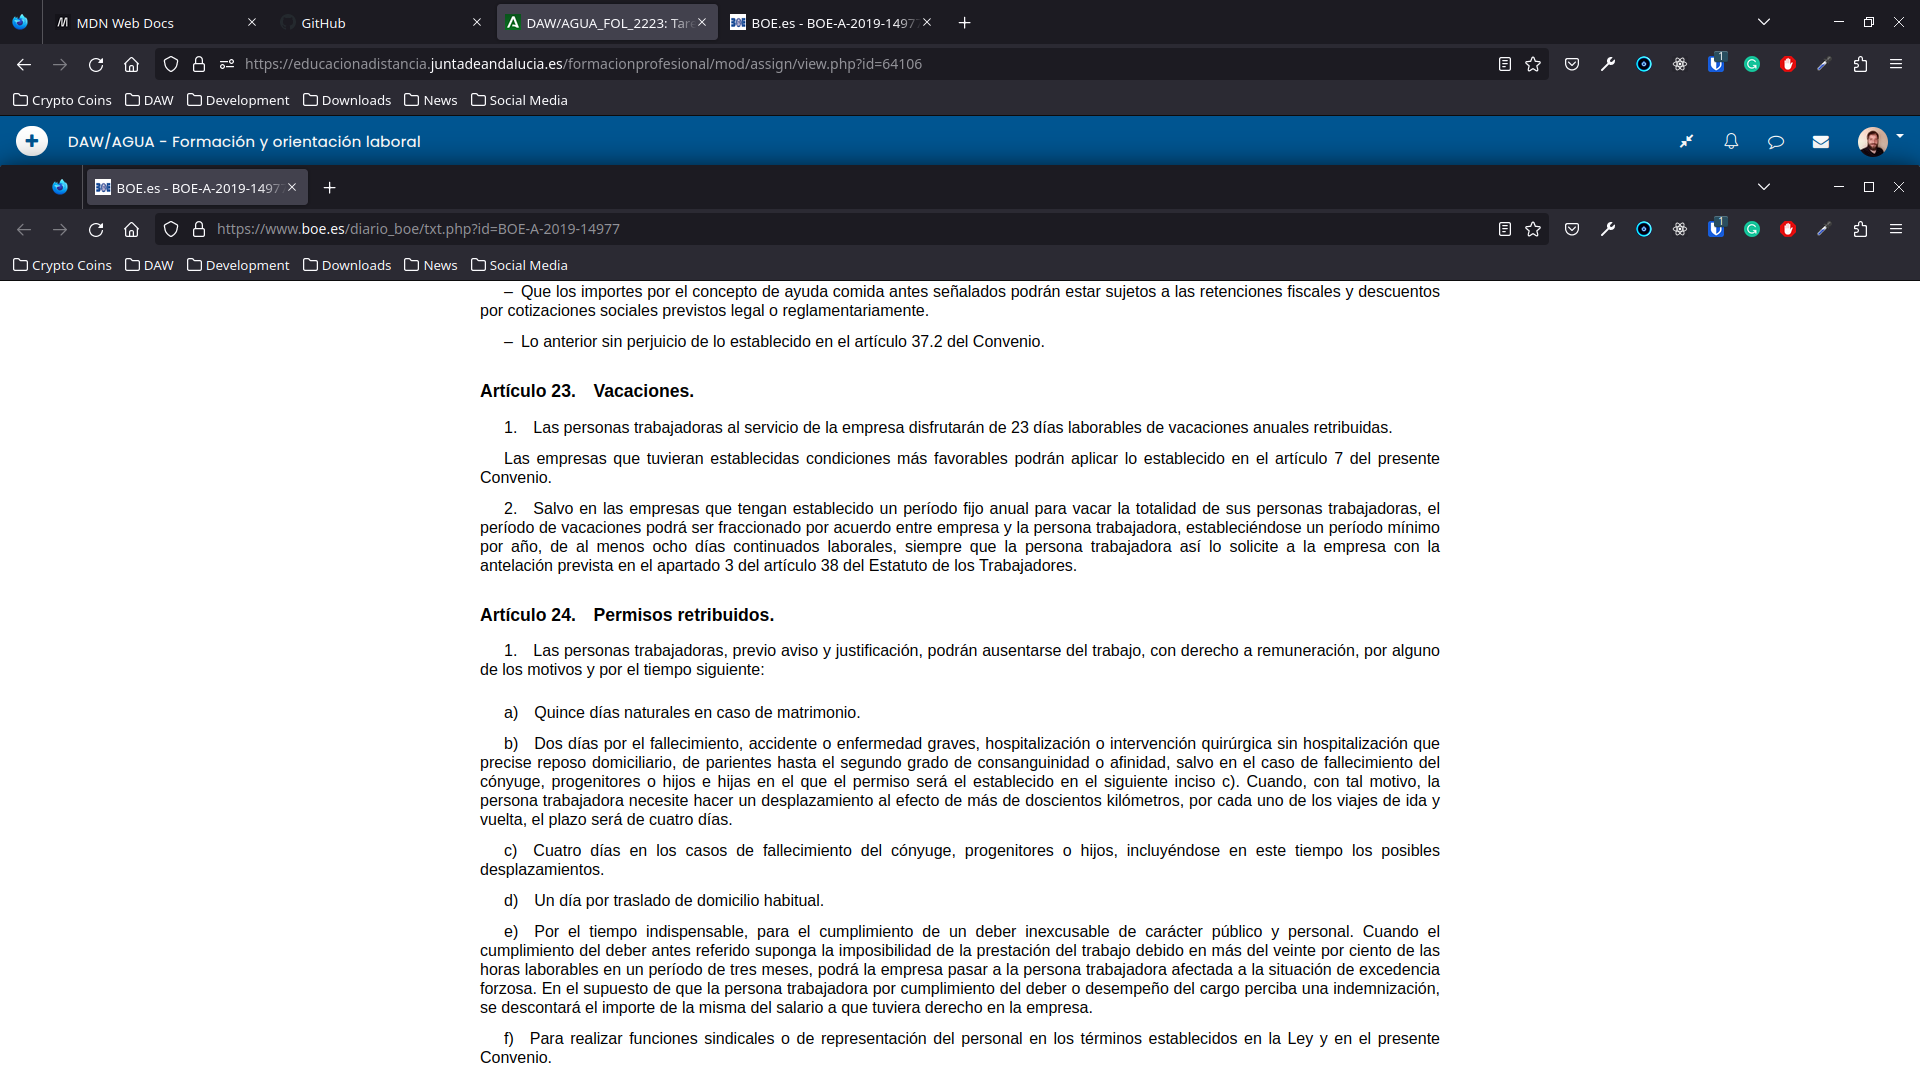
\includegraphics[scale=0.19]{conv-Vaca.png}
            \caption{Normativa sobre las vacaciones en el convenio}
        \end{figure}

        Siendo el \textbf{texto} sobre este tema el siguiente:

        \begin{itemize}
            \item \textbf{Artículo 23. Vacaciones.}
            \begin{enumerate}
                \item Las personas trabajadoras al servicio de la empresa disfrutarán de 23 días laborables de vacaciones anuales retribuidas.

                Las empresas que tuvieran establecidas condiciones más favorables podrán aplicar lo establecido en el artículo 7 del presente Convenio.

                \item Salvo en las empresas que tengan establecido un período fijo anual para vacar la totalidad de sus personas trabajadoras, el período de vacaciones podrá ser fraccionado por acuerdo entre empresa y la persona trabajadora, estableciéndose un período mínimo por año, de al menos ocho días continuados laborales, siempre que la persona trabajadora así lo solicite a la empresa con la antelación prevista en el apartado 3 del artículo 38 del Estatuto de los Trabajadores.
            \end{enumerate}
        \end{itemize}
    \end{enumerate}
\end{enumerate}








% Bibliography

\newpage
\bibliography{citas}
\bibliographystyle{unsrt}

\end{document}